Data stream is a very important concept in a modern connected Internet 
world, and it has attracted the attention of researchers worldwide. Given some important
applications of data streams, such as IoT, social networks, surveillance, and etc.,
mining data streams is becoming a more and more important topic to explore. 
However, data stream mining is also a challenging task due to its distinctive nature. 
For example, a data stream is theoretically infinite in length, therefore its volume
is very large. Meanwhile, it is possible that we have high velocity of data arrivals as well. Those properties has distinguished data 
stream mining significantly from traditional data mining problems \cite{haque2016SAND}.


% This paragraph talks about stream classification
Classification techniques solve problems of identifying which of a certain set of categories
that a new instance belongs. Normally it is assumed that the classification model, which is
trained by source data with true labels, is also representative to target data.
However, this assumption doesn't always hold in real world applications. Since data streams are generated
by non-stationary processes, it is possible that arbitrary changed may be introduced to data streams during generation. 
Due to this shift in concept, using model trained by old source data may introduce bias
in prediction \cite{herlihy1993methodology}.
In this case, a classification model trained by previous data is no longer representative to test
data in the future, and will perform poorly in prediction due to bias. Thus, the model needs regular updates to adapt the current concept.
When it comes to the setting of multistream, the classification problem becomes even
more challenging. This problem setting is described and motivated by a Multistream
Classification (MSC) algorithm \cite{chandra2016adaptive}. Two data streams are
involved simultaneously under this setting. One is referred as the source stream,
which contains data instances with true output values generated from a non-stationary
process. The other is referred as the target stream, which consists data generated
from another non-stationary process. Since getting true labels for target streams needs tremendous validation by human experts, here
we assume that true labels of test stream will not be available after the prediction. This is another assumption that previous research may suffer. 

% This paragraph talks about domain adaptation
We consider a domain adaptation setting within the multistream classification framework. there is a need to address machine learning tasks of building 
models in a one domain by using information available from another domain. In
this case, knowledge from the source domain can be transferred to the target domain to
help get high prediction accuracy. This transferring process is important in many 
circumstance where labels in a certain domain are limited or too expensive to obtain \cite{arnold2007comparative, hoi2014libol}, which fits the need of multistream by nature.
For example, it is difficult to collect labeled sensor
data from personal devices, while rich information from social media messages are available, such as 
activities and locations. Thus, knowledge from social media side can be transferred to
the physical world to address the ubiquitous computing tasks \cite{wei2016instilling}. 

In practice, most existing approaches usually conduct the learning problems in batch, such as previous example, Here, it 
assumes that training data are provided as a whole in advance \cite{pan2010survey}. However, such assumption 
doesn't always hold in real world applications, since under a data stream setting 
all instances may arrive in a sequential manner. Take online spam email detection for example \cite{chen2015opinion}. 
Normally, a classifier is built in by using a static training dataset, and it is trained in batch to
detect spam emails as accurately as possible. However, the very definition of spam varies from 
person to person. In this case, the transfer of knowledge to personalize the spam detector for each 
individual becomes critical. Even for a specific person, the definition of spam could change over time. During a 
time period one may consider advertisement from Zillow to be spam. When he starts to consider buying a house,
Zillow ads is not spam for him anymore. Such problem can be formulated as an multistream learning task, the 
objective of which is to build an online prediction model for the target domain by using information 
available in the source domain with distinct feature space. Compared to the previous example, this task 
is more challenging, as the concept is evolving in the data streams simultaneously in both source and target streams.

\begin{figure}[t]
\centering
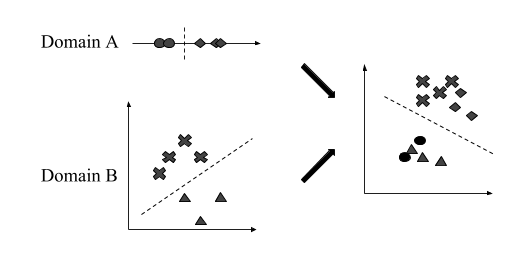
\includegraphics[width=1.0\columnwidth]{Figures/feature_projection.png}
\caption{Feature Space Projection}
\label{fig:featureprojection}
\end{figure}

This paper proposes a solution, called MultiStream Domain Adaptation (MSDA), to handle the issues described above. The
main idea is to find a common feature subspace for two distinctive streams. This idea can
be demonstrated in Figure ~\ref{fig:featureprojection}. In this case, data in domain A are 1D and in domain B are 2D. By applying the proposed projection algorithm, we
try to find a latent feature space that distribution in original and latent feature space are similar. 
Meanwhile the structure of data is preserved, which means distinct classes are still far apart.
Thus the core problem here is to find a feature space that maximize the similarity between 



